\documentclass[11pt]{article}
\usepackage[margin=1in]{geometry}
\usepackage{amsmath,amssymb,booktabs,graphicx,setspace,caption,hyperref}
\usepackage[T1]{fontenc}
\usepackage{mathpazo}
\setlength{\parindent}{0pt}
\setlength{\parskip}{0.6em}
\captionsetup{font=small,skip=6pt}
\title{Panel MS-AR(1) after a common random-walk trend\\[0.4em]\large Seasonally adjusted real GDP per worker}
\author{}
\date{}
\begin{document}
\maketitle
\section{Model}
Two-step. Step 1 builds a \emph{common} trend from average growth of countries observed in consecutive quarters (not from the level mean, which falls when poorer countries enter). Log seasonally adjusted real GDP per worker, 2026-09-17 vintage, from 1987Q1 onward.
\begin{align}
\Delta\tau_t &= \frac{1}{n_t^{\mathrm{cont}}}\sum_{i\in C_t\cap C_{t-1}} (y_{it}-y_{i,t-1}), \\
\tau_t &= \tau_{t_0}+\sum_{s=t_0+1}^{t}\Delta\tau_s.
\end{align}
The level of $\tau$ is pinned to the balanced-core mean at $t_0$. Mean $\Delta\tau$ is 0.0045 per quarter (3 countries present in every quarter). Step 2 is estimated on $y_{it}^\ast=y_{it}-\hat\tau_t$, with no extra $gt$:
\begin{align}
y_{it}^\ast &= a_i + b_i\,\lambda^{t-T_{i0}} + z_{it}, \\
a_i &\sim \mathcal{N}(\alpha,\omega^2),\qquad b_i \sim \mathcal{N}(0,\omega_b^2) \ \text{independent}, \\
z_{i,t+1} &= \bigl(1-\rho(s_{it})\bigr)\mu(s_{it}) + \rho(s_{it})\, z_{it} + \sigma(s_{it})\,\varepsilon_{it}.
\end{align}
$\lambda=0.98$ is fixed (Barro 2\% per year). $|\rho|<0.95$. Three regimes; median $\mu$ pinned at 0; $\sigma$ and $\rho$ switch. $T_{i0}$ is country $i$'s first observation after filters. Random effects: 7$\times$7 Gauss--Hermite. Plotted cycles use posterior-mean $a_i$ and $b_i$. The common trend $\tau_t$ is discarded for the structural MS-AR. Standard errors ignore step-1 uncertainty.
\begin{figure}[h]
\centering
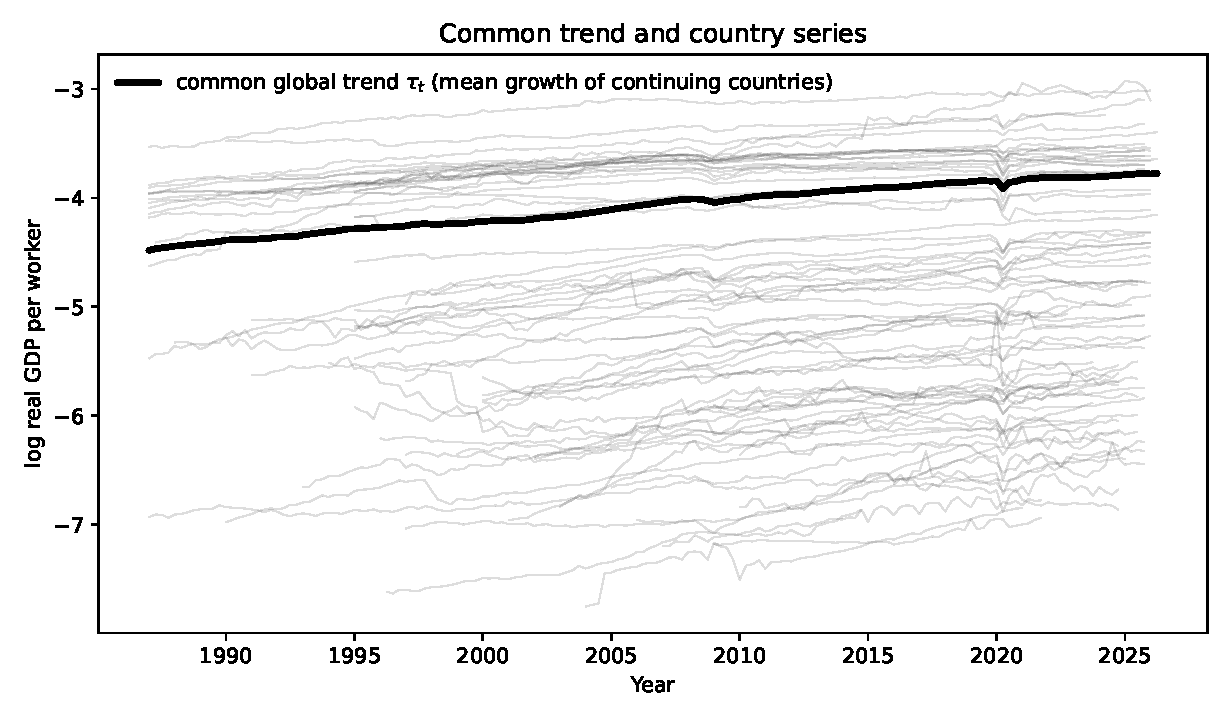
\includegraphics[width=0.88\textwidth]{figs/tau_rw.pdf}
\caption{Faint lines: country log real GDP per worker. Thick line: common $\tau_t$ from average growth of continuing countries (new entrants do not shift the level).}
\end{figure}
\clearpage
\section{Common RW trend removed; RE intercepts plus Barro catch-up}
2026-09-17 SA panel, $y_{it}-\hat\tau_t$, from 1987. 74 countries, 8291 observations, 1987-Q1--2026-Q2. $|\rho|<0.95$, $\lambda=0.98$ fixed. Fitted countries: 74. Observations: 8291. Log-likelihood: 22145.54. Ergodic mean of the cycle $E[z]=0.0465$ (0.0093).
Permanent RE intercepts and catch-up $y_{it}=a_i + b_i\lambda^{t-T_{i0}}+z_{it}$ with $\alpha=-1.0050$ (0.0132), $\omega=0.4508$ (0.0023), $\lambda=0.9800$ (fixed), $\omega_b=0.2696$ (0.0024). Posterior-mean $a_i$: mean -1.173, min -2.696, max 0.686. Posterior-mean $b_i$: mean 0.015, min -1.011, max 1.011.
\begin{table}[h]
\centering
\caption{Regime AR(1), transition matrix, and ergodic $\pi$. Columns are regimes.}
\begin{tabular}{lccc}
\toprule
 & (0) & (1) & (2) \\
\midrule
$\mu$ & -0.0326 & 0.0000 & 0.0947 \\
 & (0.0507) & --- & (0.0148) \\ \addlinespace
$\sigma$ & 0.0781 & 0.0206 & 0.0081 \\
 & (0.0039) & (0.0008) & (0.0002) \\ \addlinespace
$\rho$ & 0.9498 & 0.9500 & 0.9500 \\
 & (0.0010) & (0.0000) & (0.0000) \\ \addlinespace
$\Pi_{0\cdot}$ & 0.6688 & 0.3231 & 0.0081 \\
 & (0.0410) & (0.0451) & (0.0142) \\ \addlinespace
$\Pi_{1\cdot}$ & 0.0471 & 0.8991 & 0.0537 \\
 & (0.0076) & (0.0102) & (0.0072) \\ \addlinespace
$\Pi_{2\cdot}$ & 0.0081 & 0.0361 & 0.9558 \\
 & (0.0029) & (0.0054) & (0.0046) \\ \addlinespace
$\pi$ & 0.0713 & 0.4130 & 0.5157 \\
 & (0.0097) & (0.0238) & (0.0275) \\ \addlinespace
\bottomrule
\end{tabular}
\end{table}
\begin{figure}[h]
\centering
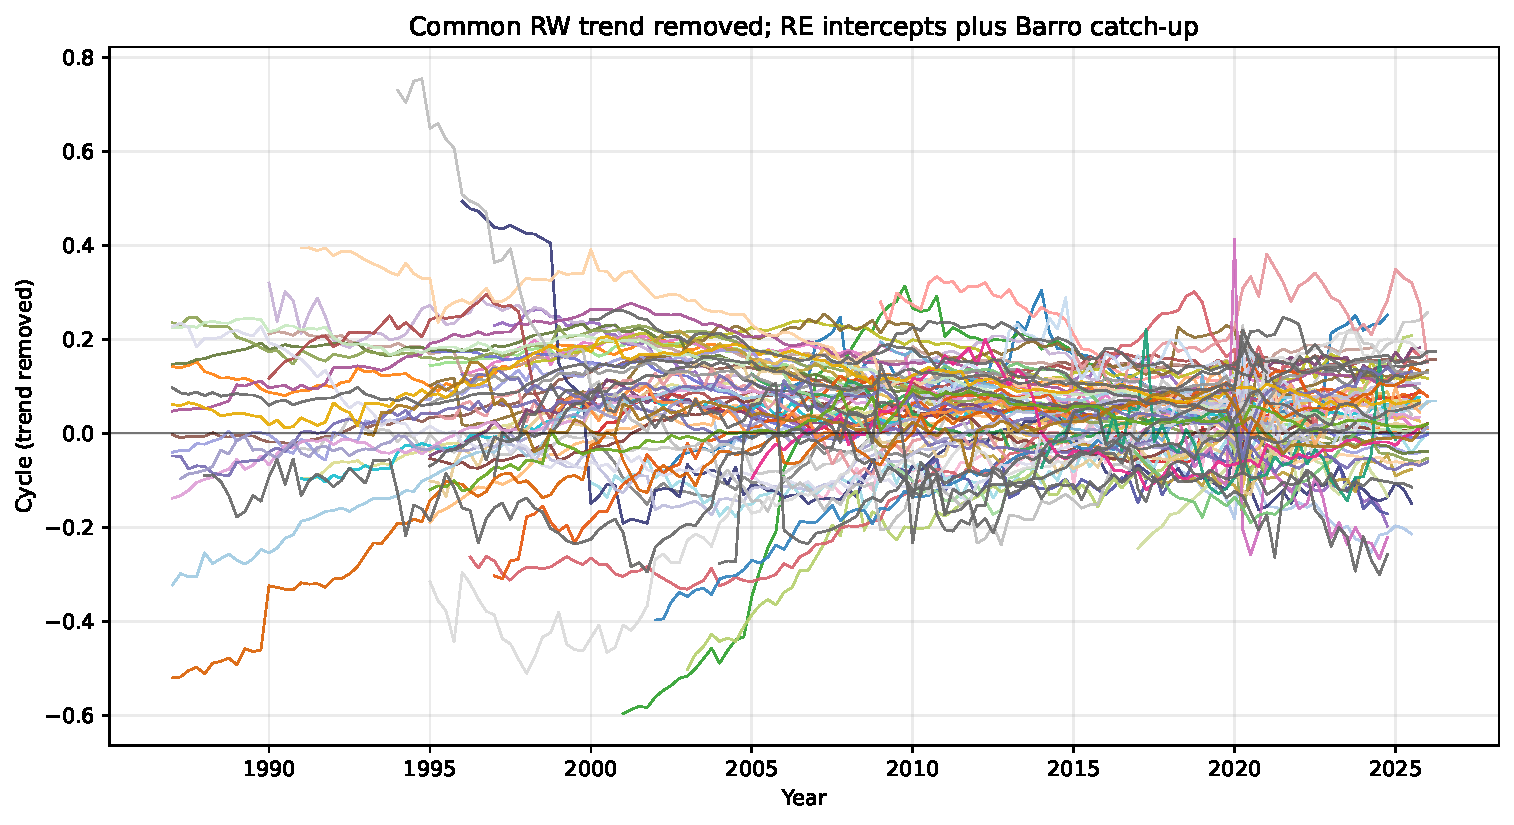
\includegraphics[width=0.75\textwidth]{figs/cycle_rw_barro.pdf}
\caption{Country cycles after removing $\tau_t$, $a_i$, and $b_i\lambda^{t-T_{i0}}$.}
\end{figure}
\end{document}
